\documentclass[12pt, letterpaper]{article}
\usepackage{bbold}
\usepackage{indentfirst}
\usepackage{amsmath, amssymb}
\usepackage[T1]{fontenc}
\usepackage[utf8]{inputenc}
\usepackage{physics}
\usepackage{tensor}
\usepackage{braket}
\usepackage{graphics}
\usepackage{grffile}
\usepackage{graphicx}
\usepackage[export]{adjustbox}

\begin{document}
    \section*{AIMD Simulation Method}
    AIMD simulations that make use of the Vienna ab initio simulation package's implementation of the density functional theory based on plane waves. It was cut 
    off at 400 eV for the plane-wave basis set. The projected augmented-wave approach was used to represent the electron-ion interaction, and generalized gradient approximation
    in the Pedrew-Bruke-Ernzerhof (PBE) from the exchange correlation were examnied. $\Gamma$ - point
    sampling were used in this method. A cubix unit cell in a eriodic boundary conditions with 100 atoms in a super cell were used. \\ 

    

    We create a script of vasp using vaspkit. After that we change parameters to PREC=N, NSW=150/200/400/500 in INCAR script file and turn on molecular 
    dynamics by USING MDALGO=2 in INCAR file.The Nose-Hoover Thermostat

    \begin{equation}
        \mathcal{L} = \sum_{i = 1}^{N} \frac{m_{i}}{2}s^{2}\dot{r_{i}}^{2} - U(r) + \frac{Q}{2}\dot{s}^{2} - gk_{B}Tln(s)   
    \end{equation}
    was used in the NVT ensemble to regulate temperature during all of the dynamic simulations. Verlet's approach was used to integrate Newton's equation of motion 
    in the velocity domain with a time step of 3 fs and a total of 600 time steps.
    The Verlet alogorithm is descibed below
    
    \begin{equation}
        \begin{split}
            \vec{v}_{N+(1/2)} &= ((1-\mu/2)\vec{v}_{N-1/2}-2\alpha \vec{F}_{N})/(1+\mu/2) \\ 
            \vec{x}_{N+1} & = \vec{x}_{N} + \vec{v}_{N+1/2}
        \end{split}
    \end{equation}
    For a seamless refining of the structure, we first loosened the structures. To 
    attain thermal equilibrium, the liquid samples of the chosen materials were first prepared at 2000K, which is much higher than their melting points. 500 steps of
    MD were user to extract quantities for pair correlation function. An equation that describes density varies as a function of a distance from a reference particle.
    
    \begin{equation}
        g(r[i]) = \frac{n_{pair}[i]}{v[i]} * \frac{V}{N_{pair}}
    \end{equation}
    Then we run simulation using the same machine, and obstained the pair correlation functions of selected materials. Thwn we reduce temperature gradually(from 2000K 
    , 1900K, 1800K, 1700K, 1600K, 1500K, 1400K, 1300K, 1200K, 1100K, 1000K, 900K, 800K, to desired temperature used in previous experiement).  

    \begin{adjustbox}{center,nofloat=figure,vspace=\bigskipamount}
        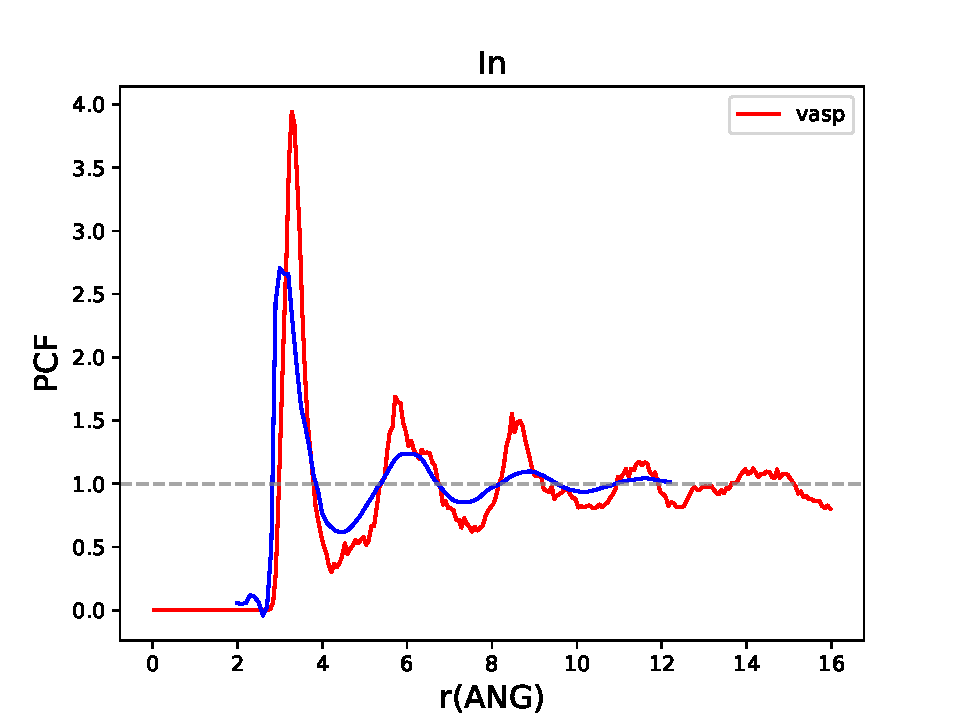
\includegraphics[width=0.5\textwidth]{pc.pdf}
        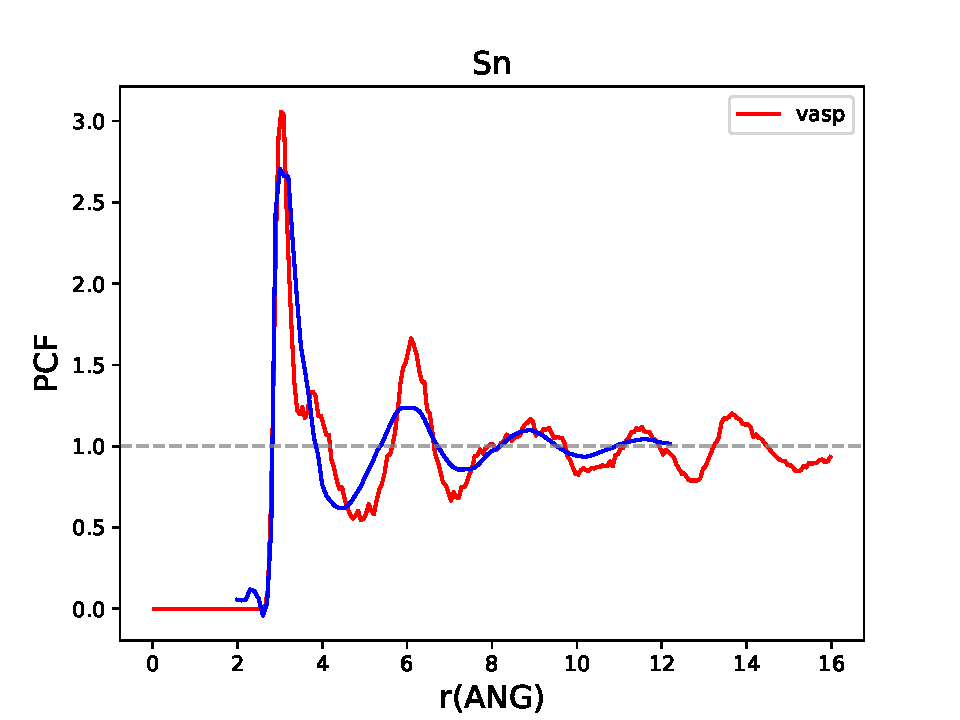
\includegraphics[width=0.5\textwidth]{Sn.pdf}
    \end{adjustbox}

    \begin{adjustbox}{center,caption={Shows pair correlation fucntions of various liquid metals},label={somelabel},nofloat=figure,vspace=\bigskipamount}
        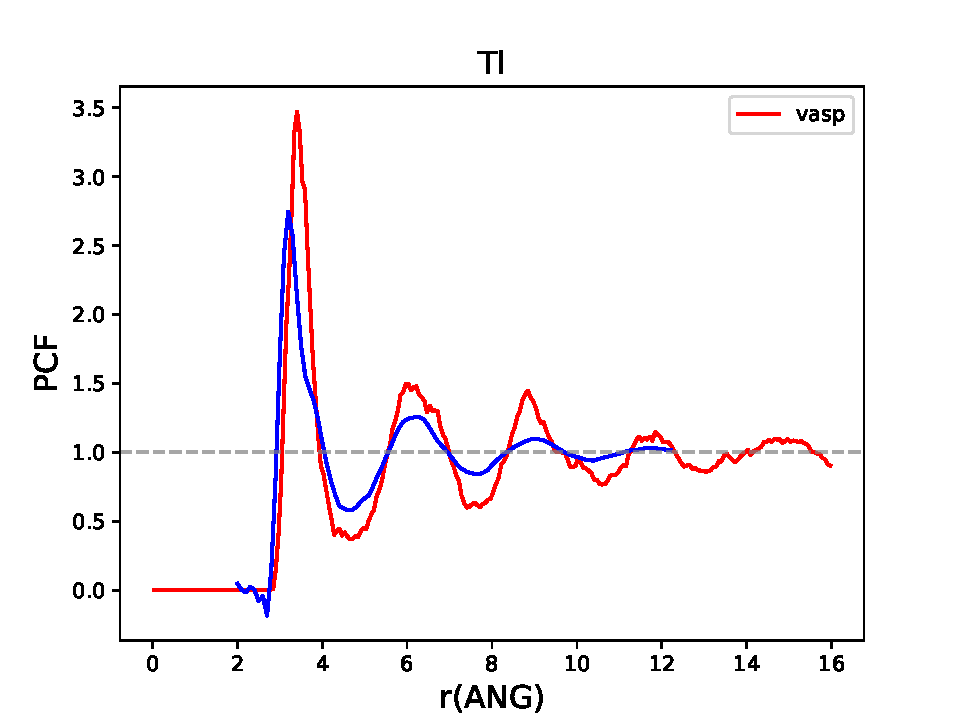
\includegraphics[width=0.5\textwidth]{Tl.pdf}
    \end{adjustbox}
\end{document}